

\documentclass[a4paper]{article}

\usepackage[english]{babel}
\usepackage[utf8x]{inputenc}
\usepackage{amsmath}
\usepackage{graphicx}
\usepackage[colorinlistoftodos]{todonotes}

\title{Présentation du stage}
\author{Guillaume Maitrot}

\begin{document}
\maketitle

\begin{center}
\centering
\title{Consommation énergétique des systèmes embarqués}
\end{center}

\section{Contexte du stage}

\subsection{Le sujet de mon stage :}
\paragraph{La consommation énergétique des systèmes embarqué }

\subsection{l'entreprise IRCICA}
\paragraph{L’Institut de Recherche en Composants logiciels et matériels pour l’Information et la Communication Avancée (IRCICA) est une Unité de Service et de Recherche (USR-3380) associant le CNRS et l’Université Lille1, sciences et technologie.
Fonctionnant comme un ‘hôtel à projets’, l’IRCICA associe environ 120 enseignants-chercheurs, chercheurs, étudiants, ingénieurs et techniciens de quatre laboratoires partenaires}

\subsection{Mon tuteur de stage :}
\subsubsection{Son profil}
    \paragraph{Mon tuteur de stage s’appelle Julien Forget , il est dans l’équipe DART mais il est aussi un Maître de Conférences à l'Université de LILLE1.}
    
\subsubsection{Coordonnées}
    \paragraph{Dans le bâtiment de l'IRCICA il se trouve au premier étage à gauche du secretariat,bureau 131.}
    
 \subsubsection{Le travail à réaliser}
    \paragraph{L'objectif du stage est de comprendre comment le logiciel consomme, i.e.
obtenir une représentation de la consommation de ce logiciel.} 
    
\subsection{Mes tâches :}
\begin{enumerate}
\item {Prise en main de la plateforme : compilation de code C pour la carte STM32, découverte de FreeRTOS}
\item {Programmation des périphériques de la carte : port série,
convertisseur Analogique-Numérique, carte mémoire flash}
\item {Développement des traitements nécessaires à l'application de
traitement du signal : acquisition de signal via le convertisseur,
traitement par une FFT, stockage du résultat de la FFT sur la carte
flash}
\item { Programmation multi-threadée de l'ensemble sous FreeRTOS}
\item {Mesure de la consommation de l'application à l'aide l'Agilent
N6705}
\item {Expérimentation sur les possibilité de variation de fréquence sur la
STM32 concernant le processeur et les périphériques}
\item {Etude des variations de la consommation selon plusieurs paramètres :
fréquence des tâches, fréquence du processeur, fréquence des
périphériques}
\end{enumerate}

\subsection{Les blocages}
\subsubsection{En cours}
    \paragraph{Mon manque de connaissance en électronnique. Je ne connaissais au départ rien de la carte STM32f4-discovery et le FreeRTOS,ce qui m'a conduit a des recherches sur le net et de quelques tutoriels simples "comme allumer une led".Après on m'a rajouter une carte flash DM-stf-4BB pour faire un discovery-kit qui entraîne des nouveaux branchements inconnus pour communiquer avec la carte flash.}
\subsubsection{à venir}
    \paragraph{La FFT me semble un peu complexe dans la pratique ,mais je comprends l'idée.}
    
\subsection{Mon environnement}
    \paragraph{On m'a installe dans le bureau 132 de l'IRCICA à côté de mon tuteur de stage qui lui est au bureau 131 ,dans mon travail je suis accompagné par quatre personnes : Julien Forget mon tuteur de stage , Alexandre Boé Maître de Conférences - Université de LILLE1 ,Giuseppe Lipari Professeur des Universités, Université de Lille et Thomas Vantroys Maître de Conférences - Université de LILLE1.Je partage mon bureau avec quatre doctorants.J'utilise un ordinateur sous ubuntu,et je reprends le projet de l'année dernière d'un autre stagiaire.}
    
\subsection{Ma première semaine de stage}
    \paragraph{La première journée j'ai fait connaissance avec le bâtiment , ainsi des quatre personnes qui m'encadrent.J'ai repris le travail de mon prédécesseur pour voir comment marche la carte, pour ensuite arrive à faire clignoter la led. Les jours suivants j'apprenais à me servir de la carte grâce aux documentations sur internet.Pour ainsi faire fonctionner un ADC et de l'USART,et la communication par spi d'une carte flash pour pouvoir enregistrer des données.   }

\section{Comment accéder au bâtiment d'IRCICA} 

\subsection{Adresse :}

    \paragraph{CAMPUS Haute-Borne CNRS IRCICA-IRI-RMN}
    \paragraph{Parc Scientifique de la Haute Borne}
    \paragraph{50 Avenue Halley}
    \paragraph{BP 70478}
    \paragraph{59658 Villeneuve d’Ascq Cédex}


\subsection{Accés pour les visiteurs}
\subsubsection{Consignes}
\begin{enumerate}
\item Vous devez vous présenter au secrétariat, le matin de 8H30 à 12h30 ou, l’après midi de 14h00 à 16h30.
\item Vous devez demander au responsable (secrétaire) d'appeler Julien Forget pour qu'il vous prenne sous sa responsabilité, de plus vous devrez porter un autocollant "visiteur".
\end{enumerate}

\subsection{Accès par autoroute}

\begin{figure}[!ht]
\centering
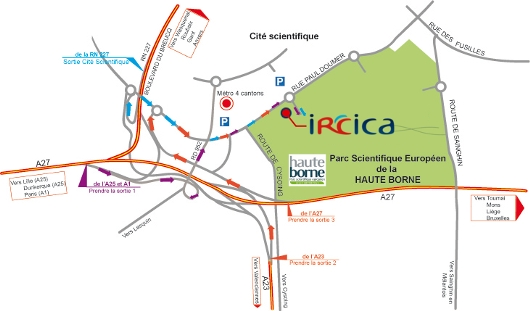
\includegraphics[width=0.8\textwidth]{acces-IRCICA-HB.jpg}
\caption{\label{fig:IRCICA}Comment accéder à IRCICA.}
\end{figure}

\end{document}